% Date : ??/??/2022
% Version : 4
% Auteur : Chahira
% Relu : 
% Relecteur : J.Roussel

% ------------------------------------------------------------ %
% ----------------------  Fiche THM01  ----------------------- %
% Thème : Gaz parfait
% Classes : toutes les classes
% ------------------------------------------------------------ %


% ======================================================= % 
% ============== Gestion de la compilation ============== %
% ======================================================= % 
\ifdefined\mainIsLoaded\else
\RequirePackage{import}
\subimport{../../}{_preambule_CdE_PC}
\begin{document}
\fi

% ======================================================= % 
% ======================================================= % 


% ===================== Couleurs ======================== %
% ======================================================= % 

% -----------------------------------%
% La commande \couleurNBouCouleur prend deux paramètres :
% #1 est la couleur NB ; #2 est la couleur "en couleur"
\def\JRLblueF{\couleurNBouCouleur{gray}{blue!50}}
\def\JRLorange{\couleurNBouCouleur{gray}{orange}}
\def\JRLgreen{\couleurNBouCouleur{gray}{green!70!blue}}
\def\JRLred{\couleurNBouCouleur{gray}{red!90!green}}
\def\JRLblueCC{\couleurNBouCouleur{lightgray!10}{blue!8}}
\def\JRLblue{\couleurNBouCouleur{black}{blue!75}}
\def\JRLblueC{\couleurNBouCouleur{lightgray!30}{blue!15}}
\def\JRLcyan{\couleurNBouCouleur{gray}{cyan}}
\def\JRLcyanC{\couleurNBouCouleur{lightgray!30}{cyan!10}}
\def\JRLbrownC{\couleurNBouCouleur{white}{brown!17.5!white}}

% ======================================================= % 


% ============================================================================ %
%                            FICHE D'ENTRAÎNEMENT                              %
% ============================================================================ %
% ======================= Métadonnées sur la fiche =========================== %
\titreFicheEntrainement		{Gaz parfaits}
\grandTheme					{Thermodynamique}
\numeroFiche				{THM01}
\uniqueID					{AGYQdPQBWkd} % une chaîne de caractères (a-z, A-Z) aléatoire de 10 caractères.
\nombreColonnesReponses		{3} % 1, 2, 3, etc.
% ============================================================================ %

%%%%%%%%%%%%%%%%%%%%%%%%%%%%%%%%%%%%%%%%%%%%%%%%%%%%%%%%%%%%%%%%%%%%%%%%%%%%%%%%%%%%%%%%%%%%%%
\debutFicheEntrainement                                                                      %
%%%%%%%%%%%%%%%%%%%%%%%%%%%%%%%%%%%%%%%%%%%%%%%%%%%%%%%%%%%%%%%%%%%%%%%%%%%%%%%%%%%%%%%%%%%%%%


% --------------------------------------------------------------------- %
%                              Prérequis                                %
%                             (facultatif)                              %
% --------------------------------------------------------------------- %
% ================== Métadonnées sur le prérequis ===================== %
\avecPrerequis{Y} % Y ou N
% ===================================================================== %
\begin{prerequis}
La loi des gaz parfaits s'écrit $PV=nRT$, avec $P$ en pascals, $V$ en mètres cubes, $n$ en moles et $T$ en kelvins.

\constantesUtiles
\begin{listeConstantes}
	\item constante des gaz parfaits : $R=\SI{8,314}{J.K^{-1}.mol^{-1}}$
	\item définition du bar : $\SI{1}{bar}=\SI{1e5}{Pa}$
	\item conversion entre kelvins et degrés Celsius : $T\,(\si{\kelvin}) = \theta\, (\si{\celsius}) + \np{273,15}$
\end{listeConstantes}
\end{prerequis}

% --------------------------------------------------------------------- %




% •••••••••••••••••••••••••••••••••••••••••••••••••••••••••••••••••••••••••••• %
% •••••••••••••••••••••••••••••••••••••••••••••••••••••••••••••••••••••••••••• %
\sectionFicheEntrainement{Entraînement au calcul}
% •••••••••••••••••••••••••••••••••••••••••••••••••••••••••••••••••••••••••••• %
% •••••••••••••••••••••••••••••••••••••••••••••••••••••••••••••••••••••••••••• %





% ********************************************************************* %
%                           ENTRAÎNEMENT                                % 
% ********************************************************************* %
% ================ Métadonnées sur l'entraînement ===================== %

\titreEntrainementFacultatif	{Quelques calculs de volume}
\hauteurLargeurCadreReponse		{7mm}{30mm}
\dureeResolutionFacultative		{2} % 1, 2, 3 ou 4
\typeEntrainement				{AN} % Newton ou QCM ou AN ou vide (exercice "normal")
\basiqueEtTransversal			{Y}
\nombreColonnesQuestions		{1} % vide, 1, 2, 3, etc.
\avecPlusieursQuestions			{Y} % Y ou N
\initialisationEntrainement
% ===================================================================== %

Calculer le volume (en \si{L}) occupé à $T=\SI{25}{\celsius}$ et sous une pression $P =\SI{1.0}{\bar}$ pour les gaz suivants.

% =============================================================================== %
\debutEntrainement
% =============================================================================== %


% ^^^^^^^^^^^^^^^^^^^^^^^^^^^^^^^^^^^^^^ %
%               Question               %
% ^^^^^^^^^^^^^^^^^^^^^^^^^^^^^^^^^^^^^^ %
\begin{enonce}
\SI{100}{g} d'argon ($M_\mathrm{Ar}=\SI{40}{g.mol^{-1}}$)	
\end{enonce}

\reponse{\SI{62}{L}}

\begin{corrige}
On a $PV=nRT$ avec $n=\frac{m}{M}$. Ainsi, on a $V=\frac{m}{M}\times \frac{RT}{P}$.
Notez que l'on peut laisser les masses en \si{g} si l'on exprime la masse molaire en \si{g.mol^{-1}}. 

Ainsi, on a
$V=\frac{\SI{100}{g} }{\SI{40}{g.mol^{-1}}}\times\frac{\SI{8,314}{J.K^{-1}.mol^{-1}}\times \SI{298.15}{K}}{\SI{1e5}{Pa}}=\SI{62e-3}{m^3}=\SI{62}{L}$.
\end{corrige}

% ************************************** %

% ^^^^^^^^^^^^^^^^^^^^^^^^^^^^^^^^^^^^^^ %
%               Question               %
% ^^^^^^^^^^^^^^^^^^^^^^^^^^^^^^^^^^^^^^ %
\begin{enonce}
\SI{32}{g} de dioxygène $\mathrm{O_2}$ ($M_\mathrm{O}=\SI{16}{g.mol^{-1}}$)	
\end{enonce}

\reponse{\SI{25}{L}}

\begin{corrige}
On a $V=\frac{\SI{32}{g}}{2\times \SI{16}{g.mol^{-1}}}\times \frac{\SI{8,314}{J.K^{-1}.mol^{-1}}\times \SI{298.15}{K}}{\SI{1e5}{Pa}}=\SI{24.8e-3}{m^3}=\SI{25}{L}$.
\end{corrige}
% ************************************** %

% ^^^^^^^^^^^^^^^^^^^^^^^^^^^^^^^^^^^^^^ %
%               Question               %
% ^^^^^^^^^^^^^^^^^^^^^^^^^^^^^^^^^^^^^^ %
\begin{enonce}
\SI{1,2}{kg} de dioxyde de carbone $\mathrm{CO_2}$ ($M_\mathrm{C}=\SI{12}{g.mol^{-1}}$)		
\end{enonce}

\reponse{\SI{6.8e2}{L}}

\begin{corrige}
On a $V=\frac{\SI{1200}{g}}{(12 + 2\times 16) \si{g.mol^{-1}}}\times \frac{\SI{8,314}{J.K^{-1}.mol^{-1}}\times\SI{298.15}{K}}{\SI{1e5}{Pa}}=\SI{0.676}{m^3}=\SI{6.8e2}{L}$.	
\end{corrige}
% ************************************** %

% =============================================================================== %
\finEntrainement
% =============================================================================== %







% ********************************************************************* %
%                           ENTRAÎNEMENT                                % 
% ********************************************************************* %
% ================ Métadonnées sur l'entraînement ===================== %

\titreEntrainementFacultatif	{Bouteille de butane}
\hauteurLargeurCadreReponse		{7mm}{3cm}
\dureeResolutionFacultative		{2} % 1, 2, 3 ou 4
\typeEntrainement				{AN} % Newton ou QCM ou AN ou vide (exercice "normal")
\nombreColonnesQuestions		{1} % vide, 1, 2, 3, etc.
\avecPlusieursQuestions			{Y} % Y ou N
\initialisationEntrainement
% ===================================================================== %

Une bouteille de \SI{30,6}{L}, maintenue à \SI{20}{\celsius}, contient du butane ($\mathrm{C_4H_{10}}$) qui est sous la forme d'un mélange liquide/gaz comprimé. Le contenu de la bouteille présente une masse $m$ de $\SI{13}{kg}$. 

On donne $M_\mathrm{H}=\SI{1}{g.mol^{-1}}$ et $M_\mathrm{C}=\SI{12}{g.mol^{-1}}$.

% =============================================================================== %
\debutEntrainement
% =============================================================================== %

% ^^^^^^^^^^^^^^^^^^^^^^^^^^^^^^^^^^^^^^ %
%               Question               %
% ^^^^^^^^^^^^^^^^^^^^^^^^^^^^^^^^^^^^^^ %
\begin{enonce}
Combien vaut la masse molaire (en $\si{g.mol^{-1}}$) du butane ?
\end{enonce}

\reponse{$\SI{58}{g.mol^{-1}}$}

\begin{corrige}
On a $M_{\mathrm{C_4H_{10}}} = 4\times M_\mathrm{C} + 10 \times M_\mathrm{H} = 4\times \SI{12}{g.mol^{-1}}+ 10 \times \SI{1}{g.mol^{-1}} = \SI{58}{g.mol^{-1}}$.
\end{corrige}

% ************************************** %


% ^^^^^^^^^^^^^^^^^^^^^^^^^^^^^^^^^^^^^^ %
%               Question               %
% ^^^^^^^^^^^^^^^^^^^^^^^^^^^^^^^^^^^^^^ %
\begin{enonce}
Quelle serait la pression à l'intérieur de la bouteille si tout le butane était à l'état gazeux ?\\\mbox{}
\end{enonce}

\reponse{\SI{1.8e2}{bar}}

\begin{corrige}
Si tout le butane était à l'état gazeux dans la bouteille et en admettant qu'il se comporte comme un gaz parfait, la pression qui y règnerait serait de 
$$
P=\frac{nRT}{V}=\frac{m}{M}\times \frac{RT}{V}=\frac{\SI{13e3}{g}}{\SI{58}{g.mol^{-1}}}\times \frac{\SI{8,314}{J.K^{-1}.mol^{-1}}\times \SI{293.15}{K}}{\SI{30.6e-3}{m^3}}
=\SI{179e5}{Pa}=\SI{1.8e2}{bar}
$$ 
et la bouteille exploserait... Heureusement qu'une grande partie est à l'état liquide !
\end{corrige}
% ************************************** %



% ^^^^^^^^^^^^^^^^^^^^^^^^^^^^^^^^^^^^^^ %
%               Question               %
% ^^^^^^^^^^^^^^^^^^^^^^^^^^^^^^^^^^^^^^ %
\begin{enonce}
Quel volume occuperait le contenu de la bouteille, s'il était entièrement à l'état gazeux, sous une pression de \SI{1.0}{bar} et à la température de \SI{20}{\celsius} ?
\end{enonce}

\reponse{\SI{5,5}{m^3}}

\begin{corrige}
En considérant le butane comme gaz parfait, on a 
\[
V=\frac{nRT}{P}=\frac{m}{M}\frac{RT}{P}=
%\frac{13}{\num{58e-3}}
\frac{\SI{13e3}{g}}{\SI{58}{g.mol^{-1}}}
\times \frac{\SI{8,314}{J.K^{-1}.mol^{-1}} \times \SI{293.15}{K}}{\SI{1e5}{Pa}}=\SI{5,5}{m^3}.
\]
\end{corrige}
% ************************************** %

% =============================================================================== %
\finEntrainement
% =============================================================================== %




% ********************************************************************* %
%                           ENTRAÎNEMENT                                % 
% ********************************************************************* %
% ================ Métadonnées sur l'entraînement ===================== %

\titreEntrainementFacultatif	{Volume molaire}
\hauteurLargeurCadreReponse		{7mm}{30mm}
\dureeResolutionFacultative		{1} % 1, 2, 3 ou 4
\typeEntrainement				{AN} % Newton ou QCM ou AN ou vide (exercice "normal")
\basiqueEtTransversal			{Y}
\nombreColonnesQuestions		{1} % vide, 1, 2, 3, etc.
\avecPlusieursQuestions			{Y} % Y ou N
\initialisationEntrainement
% ===================================================================== %

Calculer le volume molaire (en \si{L.mol^{-1}}) d'un gaz parfait :

% =============================================================================== %
\debutEntrainement
% =============================================================================== %


% ^^^^^^^^^^^^^^^^^^^^^^^^^^^^^^^^^^^^ %
%               Question               %
% ^^^^^^^^^^^^^^^^^^^^^^^^^^^^^^^^^^^^ %

\begin{enonce}
sous \SI{1.00}{bar} et à \SI{25,0}{\celsius}
\end{enonce}

\reponse{\SI{24.8}{L.mol^{-1}}}

\begin{corrige}
Le volume molaire est le volume occupé par une mole de gaz : c'est $V_\text{m}=\frac{V}{n}=\frac{RT}{P}$. 

En exprimant la pression en pascals et la température en kelvins on obtient 
\[
V_\text{m}=\frac{\SI{8,314}{J.K^{-1}.mol^{-1}}\times \SI{298.15}{K}}{\SI{1.00e5}{Pa}}=\SI{24.8e-3}{m^3.mol^{-1}}=\SI{24.8}{L.mol^{-1}}.
\]
\end{corrige}

% ************************************ %


% ^^^^^^^^^^^^^^^^^^^^^^^^^^^^^^^^^^^^ %
%               Question               %
% ^^^^^^^^^^^^^^^^^^^^^^^^^^^^^^^^^^^^ %
\begin{enonce}
sous \SI{2.00}{bar} et à \SI{50,0}{\celsius}
\end{enonce}

\reponse{\SI{13.4}{L.mol^{-1}}}

\begin{corrige}
On applique la même formule. On trouve 
\[
V_\text{m}=\frac{\SI{8,314}{J.K^{-1}.mol^{-1}}\times (\num{273.15}+50) \si{K}}{\SI{2.00e5}{Pa}}=\SI{13.4e-3}{m^3.mol^{-1}}=\SI{13.4}{L.mol^{-1}}.
\]
Remarquez que le volume molaire ne dépend pas de la nature du gaz mais seulement des conditions de pression et de température.
\end{corrige}

% ************************************ %


% =============================================================================== %
\finEntrainement
% =============================================================================== %


\newpage



% ********************************************************************* %
%                           ENTRAÎNEMENT                                % 
% ********************************************************************* %
% ================ Métadonnées sur l'entraînement ===================== %

\pointInterrogation				{Y}
\titreEntrainementFacultatif	{Surchauffe}
\hauteurLargeurCadreReponse		{7mm}{25mm}
\dureeResolutionFacultative		{1} % 1, 2, 3 ou 4
\typeEntrainement				{AN} % Newton ou QCM ou AN ou vide (exercice "normal")
\basiqueEtTransversal			{Y}
\nombreColonnesQuestions		{1} % vide, 1, 2, 3, etc.
\avecPlusieursQuestions			{N} % Y ou N
\initialisationEntrainement
% ===================================================================== %

Un pneu de voiture, de volume supposé constant, est gonflé à froid, à la température $T_{1}=\SI{20}{\celsius}$, sous la pression $P_{1}=\SI{2.0}{bar}$. Après avoir roulé un certain temps, le pneu affiche une pression $P_{2}=\SI{2.3}{bar}$. 


% =============================================================================== %
\debutEntrainement
% =============================================================================== %

% ^^^^^^^^^^^^^^^^^^^^^^^^^^^^^^^^^^^^^^ %
%               Question               %
% ^^^^^^^^^^^^^^^^^^^^^^^^^^^^^^^^^^^^^^ %
\begin{enonce}
Quelle est alors sa température (en $\si{\celsius}$) si l'on assimile l'air à un gaz parfait ?
\end{enonce}

\reponse{\SI{64}{\celsius}}

\begin{corrige}
D'après la loi des gaz parfaits : $P_{1}V=nR T_{1}$ et  $P_{2}V = nR T_{2}$ ce qui donne à volume constant : 
\[
T_{2}= T_{1} \frac{P_{2}} {P_{1}}
= (273,15+20)\si{K} \times  \frac{\SI{2.3}{bar}}{\SI{2.0}{bar}}=
\SI{337}{K}=\SI{64}{\celsius}.
\]
\end{corrige}

% ************************************** %

% =============================================================================== %
\finEntrainement
% =============================================================================== %



% ********************************************************************* %
%                           ENTRAÎNEMENT                                % 
% ********************************************************************* %
% ================ Métadonnées sur l'entraînement ===================== %

\titreEntrainementFacultatif	{}
\hauteurLargeurCadreReponse		{7mm}{25mm}
\dureeResolutionFacultative		{1} % 1, 2, 3 ou 4
\typeEntrainement				{AN} % Newton ou QCM ou AN ou vide (exercice "normal")
\basiqueEtTransversal			{Y}
\nombreColonnesQuestions		{1} % vide, 1, 2, 3, etc.
\avecPlusieursQuestions			{Y} % Y ou N
\initialisationEntrainement
% ===================================================================== %

Un récipient de volume $V_{1}$ enferme de l'air (assimilé à un gaz parfait) à la température $T_1=\SI{20}{\celsius}$ et sous une pression $P_{1}=\SI{1.20}{\bar}$. %L'air est assimilé à un gaz parfait.

Que vaut la pression finale (en bar) si l'on augmente :
% =============================================================================== %

% =============================================================================== %
\debutEntrainement
% =============================================================================== %

% ^^^^^^^^^^^^^^^^^^^^^^^^^^^^^^^^^^^^^^ %
%               Question               %
% ^^^^^^^^^^^^^^^^^^^^^^^^^^^^^^^^^^^^^^ %

\begin{enonce}
le volume de \SI{20}{\percent} ?
\end{enonce}

\reponse{\SI{1.00}{bar}}

\begin{corrige}
À température constante, le produit $PV$ reste constant d'où 
\[
P_{1}V_{1}=P_{2}V_{2}
\quad\text{avec}\quad
V_2=\num{1,2}V_1
\quad\text{d'où}\quad
P_{2}=\frac{P_1}{\num{1,2}}
=\SI{1.0}{bar}.
\]
\end{corrige}

% ************************************** %

% ^^^^^^^^^^^^^^^^^^^^^^^^^^^^^^^^^^^^^^ %
%               Question               %
% ^^^^^^^^^^^^^^^^^^^^^^^^^^^^^^^^^^^^^^ %

\begin{enonce}
la température de \SI{10}{\celsius} ?
\end{enonce}

\reponse{\SI{1.24}{bar}}

\begin{corrige}
À volume constant le quotient $P/T$ reste constant d'où
\[
\frac{P_1}{T_1}=\frac{P_2}{T_2}
\quad\text{d'où}\quad
P_{2}=P_1\frac{T_2}{T_1}=\num{1,2}\times\frac{303,15}{293,15}=\SI{1.24}{bar}.
\]
\end{corrige}

% ************************************** %

% =============================================================================== %
\finEntrainement
% =============================================================================== %





% •••••••••••••••••••••••••••••••••••••••••••••••••••••••••••••••••••••••••••• %
% •••••••••••••••••••••••••••••••••••••••••••••••••••••••••••••••••••••••••••• %
\sectionFicheEntrainement{Manipulations algébriques}
% •••••••••••••••••••••••••••••••••••••••••••••••••••••••••••••••••••••••••••• %
% •••••••••••••••••••••••••••••••••••••••••••••••••••••••••••••••••••••••••••• %


% ********************************************************************* %
%                           ENTRAÎNEMENT                                % 
% ********************************************************************* %
% ================ Métadonnées sur l'entraînement ===================== %

\titreEntrainementFacultatif	{Faire le lien entre une formule et un graphe}
\hauteurLargeurCadreReponse		{7mm}{25mm}
\dureeResolutionFacultative		{1} % 1, 2, 3 ou 4
\typeEntrainement				{} % Newton ou QCM ou AN ou vide (exercice "normal")
\nombreColonnesQuestions		{1} % vide, 1, 2, 3, etc.
\avecPlusieursQuestions			{Y} % Y ou N
\basiqueEtTransversal			{Y}
\initialisationEntrainement
% ===================================================================== %

% =============================================================================== %
\debutEntrainement
% =============================================================================== %

% ^^^^^^^^^^^^^^^^^^^^^^^^^^^^^^^^^^^^^^ %
%               Question               %
% ^^^^^^^^^^^^^^^^^^^^^^^^^^^^^^^^^^^^^^ %

\def\ratioScaleGraphe{1.2}

\begin{enonce}
Lequel de ces graphes représente la relation entre pression et température lorsque $n$ et $V$ sont fixés ?

\begin{center}
	\begin{tikzpicture}[
		scale = \ratioScaleGraphe,
		font=\footnotesize,
		every axis title/.style={below,at={(0.5,1)}}
		]
		\begin{axis}[
			title={\reponseA},
			width=40mm,
			name=plot1,
			grid=major,
			% axis y line=middle,
			% axis x line=bottom,
			axis lines=middle,% bottom,top
			inner axis line style={=>},
			xlabel style={anchor=south},
			every axis y label/.style={at={(ticklabel cs:0.5)},rotate=90,anchor=near ticklabel},
			every axis x label/.style={at={(ticklabel cs:0.5)},anchor=near ticklabel},
			xlabel={Température},
			ylabel={Pression},
			ytick=\empty,
			xtick=\empty,
			ymin=0,
			ymax=1,
			xmin=0,
			xmax=1,
			]
			\addplot+[mark=none,domain=0:1,samples=10,thick,\JRLorange]{x};
		\end{axis}
		\begin{axis}[
			title={\reponseB},
			width=40mm,
			name=plot2,at={($(plot1.east)+(1cm,0)$)},anchor=west,
			grid=major,
			% axis y line=middle,
			% axis x line=bottom,
			axis lines=middle,% bottom,top
			inner axis line style={=>},
			xlabel style={anchor=south},
			every axis y label/.style={at={(ticklabel cs:0.5)},rotate=90,anchor=near ticklabel},
			every axis x label/.style={at={(ticklabel cs:0.5)},anchor=near ticklabel},
			xlabel={Température},
			ylabel={Pression},
			ytick=\empty,
			xtick=\empty,
			ymin=0,
			ymax=1,
			xmin=0,
			xmax=1,
			]
			\addplot+[mark=none,domain=0:1,samples=50,\JRLgreen,thick]{x^2};
		\end{axis}
		\begin{axis}[
			title={\reponseC},
			width=40mm,
			name=plot3,at={($(plot2.east)+(1cm,0)$)},anchor=west,
			grid=major,
			% axis y line=middle,
			% axis x line=bottom,
			axis lines=middle,% bottom,top
			inner axis line style={=>},
			xlabel style={anchor=south},
			every axis y label/.style={at={(ticklabel cs:0.5)},rotate=90,anchor=near ticklabel},
			every axis x label/.style={at={(ticklabel cs:0.5)},anchor=near ticklabel},
			xlabel={Température},
			ylabel={Pression},
			ytick=\empty,
			xtick=\empty,
			ymin=0,
			ymax=1,
			xmin=0,
			xmax=1,
			]
			\addplot+[mark=none,domain=0:1,samples=5,thick,\JRLred]{.75};
		\end{axis}
		\begin{axis}[
			title={\reponseD},
			width=40mm,
			name=plot4,at={($(plot3.east)+(1cm,0)$)},anchor=west,
			grid=major,
			% axis y line=middle,
			% axis x line=bottom,
			axis lines=middle,% bottom,top
			inner axis line style={=>},
			xlabel style={anchor=south},
			every axis y label/.style={at={(ticklabel cs:0.5)},rotate=90,anchor=near ticklabel},
			every axis x label/.style={at={(ticklabel cs:0.5)},anchor=near ticklabel},
			xlabel={Température},
			ylabel={Pression},
			ytick=\empty,
			xtick=\empty,
			ymin=0,
			ymax=1,
			xmin=0,
			xmax=1,
			]
			\addplot+[mark=none,domain=0:1,samples=100,thick,\JRLblueF]{.1/x};
		\end{axis}
	\end{tikzpicture}
\end{center}
 \minusSmallskip
\end{enonce}

\reponse{\reponseA}

\begin{corrige}
La loi des gaz parfaits permet d'exprimer $P$ en fonction de $T$ : $P=\frac{nR}{V}T =\mathrm{C^{te}} \times T$, car $nR/V$ est constant. On prévoit donc une relation linéaire dont la courbe représentative est une droite passant par l'origine.
\end{corrige}

% ************************************** %

\bigskip
\bigskip

% ^^^^^^^^^^^^^^^^^^^^^^^^^^^^^^^^^^^^^^ %
%               Question               %
% ^^^^^^^^^^^^^^^^^^^^^^^^^^^^^^^^^^^^^^ %

\begin{enonce}
Lequel de ces graphes représente la relation entre pression et volume lorsque $n$ et $T$ sont fixés ?

\begin{center}
	\begin{tikzpicture}[
		scale = \ratioScaleGraphe,
		font=\footnotesize,
		every axis title/.style={below,at={(0.5,1)}}
		]
 		\begin{axis}[
 			title={\reponseA},
 			width=40mm,
 			name=plot1,
 			grid=major,
 			% axis y line=middle,
 			% axis x line=bottom,
 			axis lines=middle,% bottom,top
 			inner axis line style={=>},
 			xlabel style={anchor=south},
 			every axis y label/.style={at={(ticklabel cs:0.5)},rotate=90,anchor=near ticklabel},
 			every axis x label/.style={at={(ticklabel cs:0.5)},anchor=near ticklabel},
 			xlabel={Volume},
 			ylabel={Pression},
 			ytick=\empty,
 			xtick=\empty,
 			ymin=0,
 			ymax=1,
 			xmin=0,
 			xmax=1,
 			]
 			\addplot+[mark=none,domain=0:1,samples=10,thick,\JRLorange]{x};
 		\end{axis}
 		\begin{axis}[
 			title={\reponseB},
 			width=40mm,
 			name=plot2,at={($(plot1.east)+(1cm,0)$)},anchor=west,
 			grid=major,
 			% axis y line=middle,
 			% axis x line=bottom,
 			axis lines=middle,% bottom,top
 			inner axis line style={=>},
 			xlabel style={anchor=south},
 			every axis y label/.style={at={(ticklabel cs:0.5)},rotate=90,anchor=near ticklabel},
 			every axis x label/.style={at={(ticklabel cs:0.5)},anchor=near ticklabel},
 			xlabel={Volume},
 			ylabel={Pression},
 			ytick=\empty,
 			xtick=\empty,
 			ymin=0,
 			ymax=1,
 			xmin=0,
 			xmax=1,
 			]
 			\addplot+[mark=none,domain=0:1,samples=50,\JRLgreen,thick]{x^2};
 		\end{axis}
 		\begin{axis}[
 			title={\reponseC},
 			width=40mm,
 			name=plot3,at={($(plot2.east)+(1cm,0)$)},anchor=west,
 			grid=major,
 			% axis y line=middle,
 			% axis x line=bottom,
 			axis lines=middle,% bottom,top
 			inner axis line style={=>},
 			xlabel style={anchor=south},
 			every axis y label/.style={at={(ticklabel cs:0.5)},rotate=90,anchor=near ticklabel},
 			every axis x label/.style={at={(ticklabel cs:0.5)},anchor=near ticklabel},
 			xlabel={Volume},
 			ylabel={Pression},
 			ytick=\empty,
 			xtick=\empty,
 			ymin=0,
 			ymax=1,
 			xmin=0,
 			xmax=1,
 			]
 			\addplot+[mark=none,domain=0:1,samples=5,thick,\JRLred]{.75};
 		\end{axis}
 		\begin{axis}[
 			title={\reponseD},
 			width=40mm,
 			name=plot4,at={($(plot3.east)+(1cm,0)$)},anchor=west,
 			grid=major,
 			% axis y line=middle,
 			% axis x line=bottom,
 			axis lines=middle,% bottom,top
 			inner axis line style={=>},
 			xlabel style={anchor=south},
 			every axis y label/.style={at={(ticklabel cs:0.5)},rotate=90,anchor=near ticklabel},
 			every axis x label/.style={at={(ticklabel cs:0.5)},anchor=near ticklabel},
 			xlabel={Volume},
 			ylabel={Pression},
 			ytick=\empty,
 			xtick=\empty,
 			ymin=0,
 			ymax=1,
 			xmin=0,
 			xmax=1,
 			]
 			\addplot+[mark=none,domain=0:1,samples=100,thick,\JRLblueF]{.1/x};
 		\end{axis}
 	\end{tikzpicture}
 \end{center}
 \minusSmallskip
\end{enonce}

\reponse{\reponseD}

\begin{corrige}
En vertu de la loi du gaz parfait, on a $P=\frac{nRT}{V} =\frac{\mathrm{C^{te}}}{V}$, car $nRT$ est fixé. On prévoit donc une relation inverse dont la courbe représentative est une hyperbole.
\end{corrige}

% ************************************** %
% =============================================================================== %
\finEntrainement
% =============================================================================== %



\newpage


% ********************************************************************* %
%                             EXERCICE                                  % 
% ********************************************************************* %
% ================== Métadonnées sur l'exercice ======================= %
\titreEntrainementFacultatif	{Masse volumique de l'eau}
\hauteurLargeurCadreReponse		{7mm}{3cm}
\dureeResolutionFacultative		{1} % 1, 2, 3 ou 4
\typeEntrainement				{} % Newton ou QCM ou AN ou vide (exercice "normal")
\nombreColonnesQuestions		{1} % vide, 1, 2, 3, etc.
\avecPlusieursQuestions			{Y} % Y ou N
\initialisationEntrainement
% ===================================================================== %

On considère un gaz parfait de masse molaire $M$, à la pression $P$ et à la température $T$. 

% =============================================================================== %
\debutEntrainement
% =============================================================================== %

% ^^^^^^^^^^^^^^^^^^^^^^^^^^^^^^^^^^^^ %
%               Question               %
% ^^^^^^^^^^^^^^^^^^^^^^^^^^^^^^^^^^^^ %

\begin{enonce}
Exprimer sa masse volumique $\rho$ en fonction de $M$, $P$ et $T$.
\end{enonce}

\reponse{$\frac{MP}{RT}$}

\begin{corrige}
Par définition, la masse volumique vaut 
\[
\rho=\frac{m}{V}=\frac{nM}{\frac{nRT}{P}}=\frac{MP}{RT}.
\]
\end{corrige}

% ************************************ %


% ^^^^^^^^^^^^^^^^^^^^^^^^^^^^^^^^^^^^ %
%               Question               %
% ^^^^^^^^^^^^^^^^^^^^^^^^^^^^^^^^^^^^ %

\begin{enonce}
La vapeur d'eau %, qui a pour masse molaire $M_{\mathrm{H_2O}} = \SI{18}{g.mol^{-1}}$,
 a pour masse volumique $\rho=\SI{0.595}{kg.m^{-3}}$ à \SI{100}{\celsius} et $\SI{1013}{hPa}$. Sa masse molaire est $M_{\mathrm{H_2O}} = \SI{18}{g.mol^{-1}}$. \minusMedskip
  \par
Est-ce compatible avec le modèle du gaz parfait %($\mathrm{H_2O}:\SI{18}{g.mol^{-1}}$)
 ? 
\end{enonce}

\reponse{non}

\begin{corrigeNewpage}
Assimilons la vapeur d'eau à un gaz parfait : on a alors 
\[
\rho=\frac{\SI{18e-3}{kg.mol^{-1}} \times \SI{1.013e5}{Pa}} {\SI{8,314}{J.K^{-1}.mol^{-1}} \times \SI{373,15}{K}}=\SI{.588}{kg.m^{-3}}.
\] 
Ce résultat est en désaccord avec la mesure. 

Au voisinage d'un changement d'état (comme ici, où l'eau est à l'état de vapeur saturante), le modèle du gaz parfait n'est pas valide.
\end{corrigeNewpage}

% ************************************ %

% =============================================================================== %
\finEntrainement
% =============================================================================== %






% ********************************************************************* %
%                             EXERCICE                                  % 
% ********************************************************************* %
% ================== Métadonnées sur l'exercice ======================= %
\titreEntrainementFacultatif		{Compression d'un gaz}
\hauteurLargeurCadreReponse			{7mm}{3cm}
\dureeResolutionFacultative			{2} % 1, 2, 3 ou 4
\nombreColonnesQuestions			{1} % vide, 1, 2, 3, etc.
\avecPlusieursQuestions				{Y} % Y ou N
\initialisationEntrainement
% ===================================================================== %

Un gaz, initialement à la pression $P_1$ et à la température $T_1=\SI{25}{\celsius}$, est comprimé jusqu'à une pression valant $P_2=4P_1$. Sa masse volumique initiale est de $\rho_1$. 

Exprimer sa masse volumique finale $\rho_2$ en fonction de $\rho_1$ si sa température $T_2$ vaut :  

% =============================================================================== %
\debutEntrainement
% =============================================================================== %

% ^^^^^^^^^^^^^^^^^^^^^^^^^^^^^^^^^^^^ %
%               Question               %
% ^^^^^^^^^^^^^^^^^^^^^^^^^^^^^^^^^^^^ %
\begin{enonce}
$T_2 = T_1$
\end{enonce}

\reponse{$4\rho_1$}

\begin{corrige}
La masse volumique d'un gaz parfait s'écrit $\rho=\frac{MP}{RT}$. On a donc ici 
\[
\rho_1=\frac{MP_1}{RT_1}
\quad\text{et}\quad
\rho_2=\frac{MP_2}{RT_1}.
\]
Ce qui donne $\rho_2=\rho_1\frac{P_2}{P_1}=4\rho_1$.
\end{corrige}

% ************************************ %

% ^^^^^^^^^^^^^^^^^^^^^^^^^^^^^^^^^^^^ %
%               Question               %
% ^^^^^^^^^^^^^^^^^^^^^^^^^^^^^^^^^^^^ %
\begin{enonce}
$T_2 = \SI{50}{\celsius}$
\end{enonce}

\reponse{$\num{3,7}\rho_1$}

\begin{corrige}
Le même raisonnement mène à $\rho_2=\rho_1\frac{T_1P_2}{T_2P_1}=\num{3,7}\rho_1$.

{\itshape On fera attention au fait que, dans un rapport de températures, celles-ci sont à exprimer en kelvins.}
\end{corrige}
% ************************************ %

% =============================================================================== %
\finEntrainement
% =============================================================================== %





% ********************************************************************* %
%                           ENTRAÎNEMENT                                % 
% ********************************************************************* %
% ================ Métadonnées sur l'entraînement ===================== %

\titreEntrainementFacultatif	{Mouvement d'un piston}
\hauteurLargeurCadreReponse		{8mm}{3cm}
\dureeResolutionFacultative		{2} % 1, 2, 3 ou 4
\typeEntrainement				{} % Newton ou QCM ou AN ou vide (exercice "normal")
\basiqueEtTransversal			{Y}
\nombreColonnesQuestions		{1} % vide, 1, 2, 3, etc.
\avecPlusieursQuestions			{Y} % Y ou N
\initialisationEntrainement
% ===================================================================== %

Une enceinte maintenue à une température $T$ est divisée en deux parties d'égal volume $V$, par un piston mobile sans frottement. 

Initialement, le piston est bloqué, et chaque compartiment contient un gaz parfait de pressions respectives $P_1$ et $P_2$. On note $n_1$ et $n_2$ les quantités de matière dans chaque compartiment.

\begin{center}
	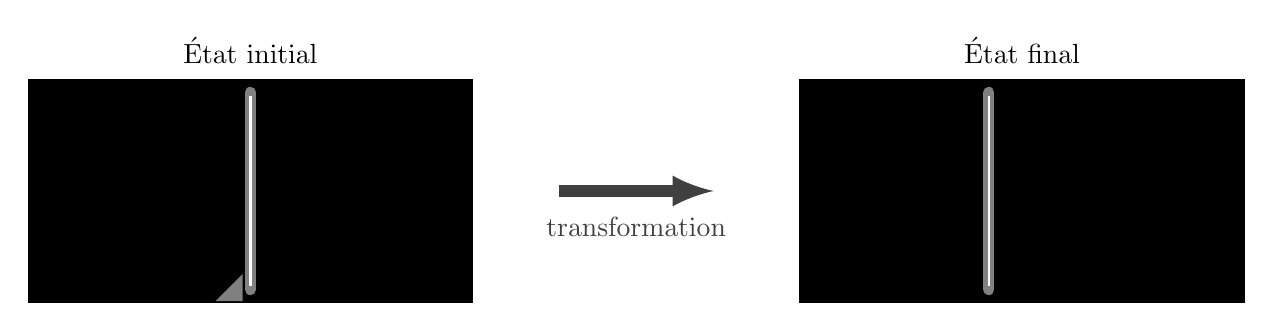
\begin{tikzpicture}[scale = 1.4]%, font=\footnotesize]
		%enceinte
		\draw[ultra thick](-2,-1)rectangle(2,1);
		%gaz
		\fill[\JRLbrownC](-2,-1)rectangle(2,1);
		% piston
		\fill[gray,shift={(-2pt,-1)}](-7pt,0)-|(0,7pt)--cycle;
		\draw[gray,line width=4pt,line cap =round] (0,-1cm+3pt)--++(0,2cm-6pt);	
		\draw[line width=1pt,white] (0,-1cm+4pt)--++(0,2cm-8pt);
		% légende
		\node at (-1,.25) {Gaz parfait};
		\node at (-1,-.1) {$P_1$, $V$, $n_1$};
		\node at (1,0.25) {Gaz parfait};
		\node at (1,-.1) {$P_2$, $V$, $n_2$};
		\node at (0,1) [above, yshift=1mm]{État initial};
		\begin{scope}[shift={(7,0)}]
%			\draw[lightgray,line width=4pt,->,>=latex,shift={(-3.5,0)}](-20pt,0)--++(40pt,0) node[midway,below=4pt]{transformation};	
			\draw[darkgray,line width=4pt,->,>=latex,shift={(-3.5,0)}](-20pt,0)--++(40pt,0) node[midway,below=4pt]{transformation};	
			%enceinte
			\draw[ultra thick] (-2,-1)rectangle(2,1);
			%gaz
			\fill[\JRLbrownC](-2,-1)rectangle(2,1);
			% piston
			\draw[gray,line width=4pt,line cap =round,shift={(-.3,0)}] (0,-1cm+3pt)--++(0,2cm-6pt);	
			\draw[line width=1pt,white,shift={(-.3,0)}] (0,-1cm+4pt)--++(0,2cm-8pt);
			% légende
			\node at (-1.2,.25) {Gaz parfait};
			\node at (-1.2,-.1) {$P'$, $V_1$, $n_1$};
			\node at (1,0.25) {Gaz parfait};
			\node at (1,-.1) {$P'$, $V_2$, $n_2$};
			\node at (0,1) [above, yshift=1mm]{État final};
		\end{scope}
	\end{tikzpicture}
\end{center}
Une fois débloqué, le piston se déplace librement de façon à ce que les pressions dans chaque compartiment deviennent égales.
\medskip

Déterminer :


% =============================================================================== %
\debutEntrainement
% =============================================================================== %

% ^^^^^^^^^^^^^^^^^^^^^^^^^^^^^^^^^^^^^^ %
%                Question                %
% ^^^^^^^^^^^^^^^^^^^^^^^^^^^^^^^^^^^^^^ %
\begin{enonce}
la relation entre $n_1$, $n_2$, $P_1$ et $P_2$
\end{enonce}

\reponse{$\frac{n_2}{n_1}=\frac{P_2}{P_1}$}

\begin{corrige}
D'après la loi du gaz parfait, on a $n_1=\frac{P_1V}{RT}$ et $n_2=\frac{P_2V}{RT}$ d'où la relation $\frac{n_2}{n_1}=\frac{P_2}{P_1}$.
\end{corrige}

% ************************************** %

% ^^^^^^^^^^^^^^^^^^^^^^^^^^^^^^^^^^^^^^ %
%                Question                %
% ^^^^^^^^^^^^^^^^^^^^^^^^^^^^^^^^^^^^^^ %
\begin{enonce}
le volume $V_1$ en fonction de $V$, $P_1$ et $P_2$
\end{enonce}

\reponse{$\frac{2P_1}{P_1+P_2}V$}

\begin{corrige}
Appliquons la loi du gaz parfait dans chaque compartiment : on a 
\[
P'V_1=n_1RT\quad\text{et}\quad P'V_2=n_2RT,
\] 
dont on déduit $V_2/V_1=n_2/n_1$. 

Par ailleurs, la conservation du volume total donne
\[
2V=V_1+V_2=V_1\left(1+\frac{n_2}{n_1}\right).
\]
Ainsi, il découle
\[
	V_1=\frac{2V}{1+n_2/n_1}=
	\frac{2V}{1+P_2/P_1}=
	\frac{2P_1}{P_1+P_2}V.
\]
\end{corrige}

% ************************************** %

% =============================================================================== %
\finEntrainement
% =============================================================================== %



\newpage




% ********************************************************************* %
%                           ENTRAÎNEMENT                                % 
% ********************************************************************* %
% ================ Métadonnées sur l'entraînement ===================== %

\titreEntrainementFacultatif	{Expression de la densité d'un gaz}
\hauteurLargeurCadreReponse		{7mm}{3cm}
\dureeResolutionFacultative		{1} % 1, 2, 3 ou 4
\typeEntrainement				{} % Newton ou QCM ou AN ou vide (exercice "normal")
\nombreColonnesQuestions		{1} % vide, 1, 2, 3, etc.
\avecPlusieursQuestions			{N} % Y ou N
\initialisationEntrainement
% ===================================================================== %

La densité $d$ d’un gaz A est le rapport entre la masse volumique du gaz A et la masse volumique de l’air sous les mêmes conditions de pression et de température. Autrement dit, c'est 
\[
d=\frac{\rho_{\ptA}}{\rho_\text{air}}.
\]
On note $M_\ptA$ la masse molaire de A et $M_\text{air}$ celle de l'air.

% =============================================================================== %
\debutEntrainement
% =============================================================================== %

% ************************************** %
% ^^^^^^^^^^^^^^^^^^^^^^^^^^^^^^^^^^^^^^ %
%               Question               %
% ^^^^^^^^^^^^^^^^^^^^^^^^^^^^^^^^^^^^^^ %
\begin{enonce}
Exprimer la densité $d$ en fonction de $M_\ptA$ et $M_\text{air}$ à l'aide de la loi du gaz parfait
\end{enonce}

\reponse{$\frac{M_\ptA}{M_\text{air}}$}

\begin{corrige}
Exprimons la masse volumique en fonction de la masse molaire pour un gaz parfait : 
\[
V=\frac{nRT}{P}=\frac{mRT}{MP}
\quad\text{donc}\quad
\rho =\frac{m}{V}=\frac{PM}{RT}.
\] Ainsi, sous la même pression et la même température, on a 
$$
d=\frac{\rho_\ptA}{\rho_\text{air}}=
\frac{PM_\ptA}{PM_\text{air}}=\frac{M_\ptA}{M_\text{air}}.
$$
\end{corrige}

% ************************************** %
% =============================================================================== %
\finEntrainement
% =============================================================================== %




% ********************************************************************* %
%                           ENTRAÎNEMENT                                % 
% ********************************************************************* %
% ================ Métadonnées sur l'entraînement ===================== %

\titreEntrainementFacultatif	{Bulle de savon}
\hauteurLargeurCadreReponse		{7mm}{4cm}
\dureeResolutionFacultative		{2} % 1, 2, 3 ou 4
\typeEntrainement				{} % Newton ou QCM ou AN ou vide (exercice "normal")
\nombreColonnesQuestions		{1} % vide, 1, 2, 3, etc.
\avecPlusieursQuestions			{Y} % Y ou N
\initialisationEntrainement
% ===================================================================== %

Une bulle de savon sphérique de rayon $r$ enferme $n$ moles d'air à la température ambiante $T_0$.   

La pression qui règne à l'intérieur de la bulle de savon est donnée par 
\[
P=P_0+\frac{4\gamma}{r}
\]
où $\gamma$ est la tension superficielle de l'eau savonneuse et où $P_0$ est la pression atmosphérique.
% =============================================================================== %


% =============================================================================== %
\debutEntrainement
% =============================================================================== %



% ^^^^^^^^^^^^^^^^^^^^^^^^^^^^^^^^^^^^^^ %
%               Question                 %
% ^^^^^^^^^^^^^^^^^^^^^^^^^^^^^^^^^^^^^^ %

\begin{enonce}
Donner l'expression du volume de la bulle en fonction $r$
\end{enonce}

\reponse{$\frac43 \pi r^3$}

\begin{corrige}
Le volume de la bulle vaut $V=\frac43 \pi r^3$.
\end{corrige}

% ************************************** %


% ^^^^^^^^^^^^^^^^^^^^^^^^^^^^^^^^^^^^^^ %
%               Question                 %
% ^^^^^^^^^^^^^^^^^^^^^^^^^^^^^^^^^^^^^^ %

\begin{enonce}
Exprimer $n$ en fonction de $P_0$, $T_0$, $\gamma$ et $r$
\end{enonce}

\reponse{$\frac{4\pi P_0r^3+16\pi\gamma r^2}{3RT_0}$}

\begin{corrige}
La pression de l'air intérieure vaut $P=P_0+\frac{4\gamma}{r}$. La loi des gaz parfaits donne alors :
\[
PV = \left(P_0+\frac{4\gamma}{r}\right) \times \frac43 \pi r^3=nRT_0
\quad\text{d'où}\quad
n=\frac{4\pi P_0r^3+16\pi\gamma r^2}{3RT_0}.
\]
\end{corrige}

% ************************************** %



% =============================================================================== %
\finEntrainement
% =============================================================================== %




 



% •••••••••••••••••••••••••••••••••••••••••••••••••••••••••••••••••••••••••••• %
% •••••••••••••••••••••••••••••••••••••••••••••••••••••••••••••••••••••••••••• %
\sectionFicheEntrainement{Mélange de gaz parfaits}
% •••••••••••••••••••••••••••••••••••••••••••••••••••••••••••••••••••••••••••• %
% •••••••••••••••••••••••••••••••••••••••••••••••••••••••••••••••••••••••••••• %

\bigskip

{\itshape Tous les mélanges de gaz seront considérés parfaits.}

% ********************************************************************* %
%                             EXERCICE                                  % 
% ********************************************************************* %
% ================== Métadonnées sur l'exercice ======================= %
\titreEntrainementFacultatif		{Un gaz sous pression}
\hauteurLargeurCadreReponse			{6mm}{2cm}
\dureeResolutionFacultative			{3} % 1, 2, 3 ou 4
\nombreColonnesQuestions			{2} % vide, 1, 2, 3, etc.
\avecPlusieursQuestions				{Y} % Y ou N
\initialisationEntrainement
% ===================================================================== %
% source : https://lelementarium.fr/focus/gaz-naturel/

Un gisement donné %de \emph{Groningen} 
fournit du gaz naturel dont la composition (en fractions molaires) est :
\begin{center}
\begin{minipage}{0.7\textwidth}
\begin{multicols}{2}
\begin{itemize}
\item
\SI{81,3}{\percent}  méthane ($\mathrm{CH_4}$)
\item
\SI{2,9}{\percent}  éthane ($\mathrm{C_2H_6}$)
\item
\SI{0,4}{\percent}  propane ($\mathrm{C_3H_8}$)
\end{itemize}
\begin{itemize}
\item
\SI{0,2}{\percent}  butane ($\mathrm{C_4H_{10}}$)
\item
\SI{14,3}{\percent}  diazote ($\mathrm{N_2}$)
\item[]
\end{itemize}
\end{multicols}
\end{minipage}
\end{center}

On donne $M_{\mathrm{H}} = \SI{1}{g.mol^{-1}}$, $M_{\mathrm{C}} = \SI{12}{g.mol^{-1}}$ et $M_{\mathrm{N}} = \SI{14}{g.mol^{-1}}$.

Calculer :
\minusSmallskip

% =============================================================================== %
\debutEntrainement
% =============================================================================== %

% ^^^^^^^^^^^^^^^^^^^^^^^^^^^^^^^^^^^^ %
%               Question               %
% ^^^^^^^^^^^^^^^^^^^^^^^^^^^^^^^^^^^^ %
\begin{enonce}
la masse molaire du mélange
\end{enonce}

\reponse{\SI{18.2}{g.mol^{-1}}}

\begin{corrige}
La masse molaire du mélange est la moyenne pondérée des masses molaires : $M=\sum_i x_iM_i$. 

Ce qui donne ici
\[
M= \big(\num{0.813}\times 16+\num{0.029}\times 30+\num{0.004}\times 44+\num{0.002}\times 58+\num{0.143}\times 28\big)~\si{{g.mol^{-1}}}=
\SI{18.2}{g.mol^{-1}}.
\]
\end{corrige}

% ************************************** %


% ^^^^^^^^^^^^^^^^^^^^^^^^^^^^^^^^^^^^ %
%               Question               %
% ^^^^^^^^^^^^^^^^^^^^^^^^^^^^^^^^^^^^ %
\begin{enonce}
la fraction massique de l'éthane
\end{enonce}

\reponse{\SI{4,79}{\percent}}

\begin{corrige}
Faisons un bilan avec une mole de mélange : 
\begin{itemize}
\item le mélange a une masse totale $m=\SI{18.2}{g}$ ;
\item ce mélange contient \SI{0.029}{mol} d'éthane soit $m_\mathrm{C_2H_6}=\num{0.029}\times 30=\SI{.87}{g}$.
\end{itemize}
On en déduit le titre massique vaut 
\[
w_\mathrm{C_2H_6}=m_\mathrm{C_2H_6}/m=\SI{4.79}{\percent}.
\]
\end{corrige}

% ************************************** %

% =============================================================================== %
\finEntrainement
% =============================================================================== %




% ********************************************************************* %
%                             EXERCICE                                  % 
% ********************************************************************* %
% ================== Métadonnées sur l'exercice ======================= %
\titreEntrainementFacultatif	{Composition d'un mélange}
\hauteurLargeurCadreReponse		{6mm}{4cm}
\dureeResolutionFacultative		{2} % 1, 2, 3 ou 4
\nombreColonnesQuestions		{1} % vide, 1, 2, 3, etc.
\avecPlusieursQuestions			{Y} % Y ou N
\initialisationEntrainement
% ===================================================================== %

Un mélange de diazote $\mathrm{N_2}$ ($M_\mathrm{N}=\SI{14}{g.mol^{-1}}$) et de dioxygène $\mathrm{O_2}$ ($M_\mathrm{O}=\SI{16}{g.mol^{-1}}$) présente une masse volumique de \SI{1,00}{g.L^{-1}} à \SI{100}{\celsius} et sous une pression de \SI{1013}{hPa}.

% =============================================================================== %
\debutEntrainement
% =============================================================================== %

% ^^^^^^^^^^^^^^^^^^^^^^^^^^^^^^^^^^^^ %
%               Question               %
% ^^^^^^^^^^^^^^^^^^^^^^^^^^^^^^^^^^^^ %
\begin{enonce}
Calculer la masse molaire du mélange
\end{enonce}

\reponse{\SI{30.6}{g.mol^{-1}}}

\begin{corrige}
Le mélange étant considéré parfait, on peut appliquer la loi du gaz parfait : 
\[
PV=nRT
\quad\text{d'où}\quad
\rho=\frac{m}{V}=\frac{MP}{RT}.
\]
On en déduit la masse molaire
\[
M=\frac{\rho RT}{P}=
\frac{\SI{1}{kg.m^{-3}}\times \SI{8,314}{J.K^{-1}.mol^{-1}} \times \SI{373,15}{K}}{\SI{1.013e5}{Pa}}=\SI{30.6e-3}{kg.mol^{-1}}.
\]
\end{corrige}

% ************************************** %


% ^^^^^^^^^^^^^^^^^^^^^^^^^^^^^^^^^^^^ %
%               Question               %
% ^^^^^^^^^^^^^^^^^^^^^^^^^^^^^^^^^^^^ %
\begin{enonce}
En déduire la fraction molaire en dioxygène
\end{enonce}

\reponse{\SI{65,6}{\percent}}

\begin{corrige}
La masse molaire du mélange est la moyenne pondérée des masses molaires. Si l'on note $x$ la fraction molaire en dioxygène et $y$ celle en diazote, on a $M=xM_\mathrm{O_2}+yM_\mathrm{N_2}$ avec $x+y=1$. On en déduit 
\[
x=\frac{M-M_\mathrm{N_2}}{M_\mathrm{O_2}-M_\mathrm{N_2}}=\frac{\SI{30.626}{g.mol^{-1}}-\SI{28}{g.mol^{-1}}}{\SI{32}{g.mol^{-1}}-\SI{28}{g.mol^{-1}}}=\SI{65,6}{\percent}.
\]
\end{corrige}

% ************************************** %

% =============================================================================== %
\finEntrainement
% =============================================================================== %








% ********************************************************************* %
%                             EXERCICE                                  % 
% ********************************************************************* %
% ================== Métadonnées sur l'exercice ======================= %
\titreEntrainementFacultatif		{Air humide}
\hauteurLargeurCadreReponse		{6mm}{4cm}
\dureeResolutionFacultative		{2} % 1, 2, 3 ou 4
\nombreColonnesQuestions		{1} % vide, 1, 2, 3, etc.
\avecPlusieursQuestions			{N} % Y ou N
\initialisationEntrainement
% ===================================================================== %

L'humidité relative (ou \emph{taux d'hygrométrie}) est le rapport 
\[
H = \frac{\text{pression partielle de vapeur d'eau}}{\text{pression de vapeur saturante}}.
\]
La pression de vapeur saturante de l'eau à \SI{25}{\celsius} vaut \np[Pa]{3166}.

\smallskip

% =============================================================================== %
\debutEntrainement
% =============================================================================== %

% ^^^^^^^^^^^^^^^^^^^^^^^^^^^^^^^^^^^^ %
%               Question               %
% ^^^^^^^^^^^^^^^^^^^^^^^^^^^^^^^^^^^^ %

\begin{enonce}
Quelle est la masse de vapeur d'eau (on donne $M_\mathrm{H_2O} = \SI{18}{g.mol^{-1}}$) présente dans une pièce de \SI{400}{m^3} contenant de l'air à \SI{25}{\celsius} un jour où l'humidité relative est de \SI{60}{\percent} ?
\end{enonce}

\reponse{\SI{5.5}{kg}}

\begin{corrige}
Calculons la pression partielle en vapeur d'eau : elle vaut $P_\mathrm{H_2O}=\SI{60}{\percent} p_\text{sat}=\SI{1.90e3}{Pa}$. 

Dans un volume de \SI{400}{m^3} cela correspond à une quantité de matière
\[
n_\mathrm{H_20}=\frac{P_\mathrm{H_2O}V}{RT}=\frac{\SI{1.90e3}{Pa}\times \SI{400}{m^3}}{\SI{8,314}{J.K^{-1}.mol^{-1}} \times \SI{298,15}{K}}=\SI{307}{mol}.
\]
Ce qui représente une masse $m=n_\mathrm{H_2O}\times M_\mathrm{H_2O}=\SI{18e-3}{kg.mol^{-1}}\times \SI{307}{mol}=\SI{5.5}{kg}$.
\end{corrige}

% ************************************** %

% =============================================================================== %
\finEntrainement
% =============================================================================== %






% ********************************************************************* %
%                           ENTRAÎNEMENT                                % 
% ********************************************************************* %
% ================ Métadonnées sur l'entraînement ===================== %

\titreEntrainementFacultatif	{Ajout d'un gaz}
\hauteurLargeurCadreReponse		{5mm}{3cm}
\dureeResolutionFacultative		{1} % 1, 2, 3 ou 4
\typeEntrainement				{} % Newton ou QCM ou AN ou vide (exercice "normal")
\nombreColonnesQuestions		{1} % vide, 1, 2, 3, etc.
\avecPlusieursQuestions			{Y} % Y ou N
\initialisationEntrainement
% ===================================================================== %

Un récipient clos de volume $V$ enferme un mélange gazeux contenant deux espèces A et B à une température $T$ fixée. La pression totale vaut $P=\SI{1500}{hPa}$ et la pression partielle de A est de \SI{1100}{hPa}.
% =============================================================================== %
\debutEntrainement
% =============================================================================== %

% ^^^^^^^^^^^^^^^^^^^^^^^^^^^^^^^^^^^^^^ %
%               Question               %
% ^^^^^^^^^^^^^^^^^^^^^^^^^^^^^^^^^^^^^^ %
\begin{enonce}
 Quelle est la pression partielle de B ? 
\end{enonce}

\reponse{$\SI{400}{hPa}$}

\begin{corrige}
La loi de Dalton impose $P=P_\ptA+P_\ptB$ d'où $P_\ptB=\SI{400}{hPa}$.
\end{corrige}

% ************************************** %

% ^^^^^^^^^^^^^^^^^^^^^^^^^^^^^^^^^^^^^^ %
%               Question               %
% ^^^^^^^^^^^^^^^^^^^^^^^^^^^^^^^^^^^^^^ %
\begin{enonce}
On ajoute une espèce C au système de sorte que la pression totale augmente jusqu'à $\SI {1800}{hPa} $. \par
Quelle est la nouvelle pression partielle de B ?
\end{enonce}

\reponse{$\SI{400}{hPa}$}

\begin{corrige}
La pression partielle d'une espèce dépend de sa quantité de matière, sa température et du volume total. 
En effet, 
\[
P=\frac{\Big (\displaystyle\sum_i {n_i}\Big )\times RT}{V}=\sum_i P_i
\quad\text{avec}\quad
P_i=\frac{n_iRT}{V}.
\]
Puisque ces quantités n'ont pas changé pour l'espèce B, sa pression partielle est restée la même.
\end{corrige}

% ************************************** %


% =============================================================================== %
\finEntrainement
% =============================================================================== %





% ---------------------------------------------------------------------------- %
%                       Affichage des réponses mélangées                       %
% ---------------------------------------------------------------------------- %
\afficheReponsesMelangees
% ---------------------------------------------------------------------------- %

%%%%%%%%%%%%%%%%%%%%%%%%%%%%%%%%%%%%%%%%%%%%%%%%%%%%%%%%%%%%%%%%%%%%%%%%%%%%%%%%%%%%%%%%%%%%%%
\finFicheEntrainement                                                                        %
%%%%%%%%%%%%%%%%%%%%%%%%%%%%%%%%%%%%%%%%%%%%%%%%%%%%%%%%%%%%%%%%%%%%%%%%%%%%%%%%%%%%%%%%%%%%%%


% ======================================================= % 
% ============== Gestion de la compilation ============== %
% ======================================================= % 
\ifdefined\mainIsLoaded\else
\printReponsesEtCorriges
\end{document}\fi
% ======================================================= % 
% ======================================================= % 
